We apply our framework and methodology on a specific problem: A puzzle assembly task. The goal is to assemble several heterogenous pieces together to create a specific final shape. This is done using a robotic platform, simulated using a realistic physics simulator: Webots~\cite{Michel:2004p10762}.

This allows us to get a measurable system which could be transformed into a real platform pretty easily.

\section{Definition of the puzzle test-case} % (fold)
\label{sec:definition_of_the_puzzle_test_case}

We define the puzzle test-case as follows:
\begin{my_itemize}
	\item Let a puzzle of square shape, with area $25$, be constructed out of 5 pieces of area 5 each with different given shapes.
	\item Let the final assembly shapes $S_k$ of this puzzle be know.
	\item Let the set of assembly plans $P_k$ leading to the final shapes $S_k$ be known. 
	\item Let the puzzle pieces assemble by bi-directional connections. One connection is enough for two pieces to be attached. These connection and their positions on the different pieces are known.
	\item Pieces can be assembled and disassembled.
	\item Piece can lie around or move randomly. We study those two possibilities, but we concentrate on the first one. 
	\item Consider an arena of sufficiently large size so that small scale interactions dynamics can be ignored.
	\item Fill this arena with $n_i$ initial pieces of each shape $i$. Let these $n_i$ number be the exact numbers needed to construct $N$ final assemblies.
	\item Consider $M$ robots, able to pick up pieces and to make them assemble and disassemble.
	\item Allow a recognition by the robots and by the pieces of the shapes and connection points when an encounter occur.
	\item \textbf{Then:}\\
	How can you manipulate those initial pieces so that after a time $T_f$, the number of assembled puzzles $X_{S_k}$ corresponds to desired values?
\end{my_itemize}

We introduced here the goal of this whole test case: to control the output of the system in term of assembled puzzles.

This can also be applied on the fly, to control what the system should produce. We want here to take advantage of the modularity of the platform, as our robots can produce any desired assembly.

An application of that flexibility can be what we call a \textit{green manufacturing} process. We mean by that the automatic recycling of finished puzzles $S_1$ to create new puzzles $S_2$, only by telling the robots what we want as final assembly. This will be studied in Chapter~\ref{cha:chemical_reaction_networks_control_and_design}.

% section definition_of_the_puzzle_test_case (end)

\section{Scale and complexity considerations} % (fold)
\label{sec:scale_and_complexity_considerations}

We have a lot of different possibilities for the robot behaviors. We chose to consider different directions depending on the available information and capabilities of the robots. If we want to produce something really scalable, then using robots as simple as possible is interesting. But on the other hand, this would most likely affect the performances. So we will try to measure this with respect to several considerations.

\begin{table}[h!]
	\begin{center}
	\begin{tabular}{r|c|c}
		& \textbf{Assembly plan known} & \textbf{Local plans only} \\
		\hline
		\textbf{Local information} & \textit{Current study} & \textit{Future work} \\
		\hline
		\textbf{Global information} & Market-based, Assembly line & Market-based
	\end{tabular}
	\end{center}
	\caption{Robot behavior depending on available informations.}
	\label{tab:robot_behavior}
\end{table}

The first distinctions we make are shown in Table~\ref{tab:robot_behavior}. The most important criteria is the availability of information about the robots and pieces positions and states. If we have a Global information state, then the problem reduces to a classical assembly at the macro-level. With multiple robots, this could be solved using Market-based strategies, which do not interest us here. So we only consider having Local information about the pieces and robots positions.

The next distinction is the availability of the full assembly plan. Knowing the full assembly allows to optimize a-priori a plan and to stick to it when building the puzzle. But this needs some computing capabilities and communications between pieces and robots. A more crude possibility is forbidding this full knowledge, and having to recreate the global plan only from local connections possibilities.

We are currently studying the \textit{Local info / Assembly plan} case. The \textit{Local info / Local plan} case is very interesting but will be done in further works.

Furthermore, we have the following choice to make: \textit{should the pieces be disassembled or not}?
As we will develop during the project, this depends on the possibility of bad assemblies and on the flexibility of creation needed. Indeed, if we want to apply our system to the \textit{green assembly} process, we have to be able to destroy final products into simpler ones.

This is in accordance with biology, which tends to reuse products and compounds for different purposes. This allows a flexibility and adaptation necessary when we do not know the goal a priori.

A quick precision should be done on the moving capabilities of pieces. We concentrate here on the task of assembling immobile pieces. In this case, the robots behaves like transporters. But, seen more abstractly, this is the same as having moving pieces on their own.
We also study the case of pieces moving around randomly. This simulates more closely a self-assembly task, driven only by geometric constraints for the assembly.
An interesting scenario is to add robots to the system with moving pieces. In this setup, the added robots behaves like enzymes: they modify the system by acting on it. This creates three different scenario: the \textit{robot-transporter}, the \textit{self-assembling pieces} and the \textit{mixed assembly}.

In all this section, we only consider forward assemblies of pieces, that is, we never disassemble things. This will be explored further on, in the Augmentation step, Chapter~\ref{cha:augmented_assembly_implementation}.
% section scale_and_complexity_considerations (end)

\section{Webots implementation} % (fold)
\label{sec:webots_implementation}
	
	We chose to develop our puzzle test case using the realistic physic simulator Webots~\cite{Michel:2004p10762}. This allows us to simulate robots and assembly process, while still being affected by noise and geometric properties. We could have developed a simpler simulator, for example a point-based simulator for an assembly process, but we think that the added physical reality of Webots makes it easier to understand how real-world problems could behave in our framework.
	
	Webots offers directly a capability to assemble our puzzle pieces: connectors. These connectors behaves like active electromagnets, that can be turned on and off. The goal is to mimic the assembly process of molecular compounds, tied by low-energy bounds.
	
	\paragraph{}
\textit{The first implementation of the controllers for the robot transporters scenario on Webots has been created by Spring Berman for her project in the course MEAM620 by V. Kumar at the University of Pennsylvania. Lo\"ic Matthey created the Webots worlds and subsequently modified the controllers code to improve scalability, add the support for arbitrary assembly plans, change the movement patterns and create the self-assembly and mixed-assembly scenarios.}
	
	\subsection{Pieces} % (fold)
	\label{sub:pieces}
	
		A piece consists of a solid body, several small feet and several connectors. There is only one top connector for the robots to carry the piece around. There are several side connectors, to connect to other pieces, their number depend on the piece type. See Figure~\ref{fig:piece_alone_overview} for an example of such a piece.		
		\begin{figure}[h]
			\centering
				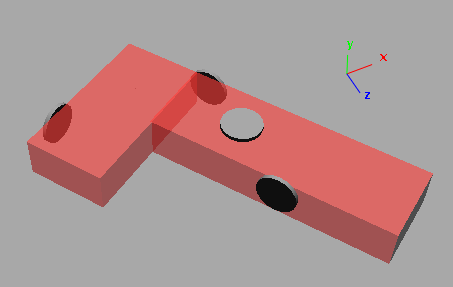
\includegraphics[width=6cm]{img/piece_alone.png}
			\caption{Piece overview. Top connector is for the robots, side connectors are for the other pieces.}
			\label{fig:piece_alone_overview}
		\end{figure}
	
		We created a set of four different pieces, each with different shapes and different connecting capabilities. See Figure~\ref{fig:pieces_types} for the different pieces.
		
		\begin{figure}[h]
			\centering
				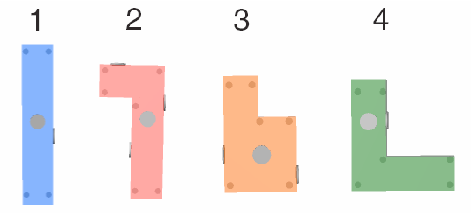
\includegraphics[width=8cm]{img/pieces_types.pdf}
			\caption{Four different pieces created, with their different connecting capabilities.}
			\label{fig:pieces_types}
		\end{figure}
		
		These pieces are endowed with several other capabilities:
		\begin{enumerate}
			\item They have a radio emitter/receiver to communicate with robots or other pieces. The communication range is set to 40cm for the pieces.
			\item They can activate or deactivate their connectors at will.
			\item They know what type they are and where are their connectors.
			\item They know the assembly plans to create the different final puzzles. They also know how they should be oriented for optimal assembly with a give other piece. We will see later that this can be relaxed.
			\item They are fairly intelligent, meaning that they have computational capabilities. The pieces can communicate with other robots, maintain a internal state of their situation.
		\end{enumerate}
		
		\subsubsection{Assembly plans} % (fold)
		\label{ssub:assembly_plans}
			We consider two final puzzles in our project. There are several way of assembling them. We first study two specific plans, but will generalize that when trying to control the chemical reactions network. The two plans and the different mid-assemblies resulting are presented in Figure~\ref{fig:assembly_plans}.
			
			\begin{figure}[h!]
				\centering
				\subfigure[First final puzzle plan] 
				{
					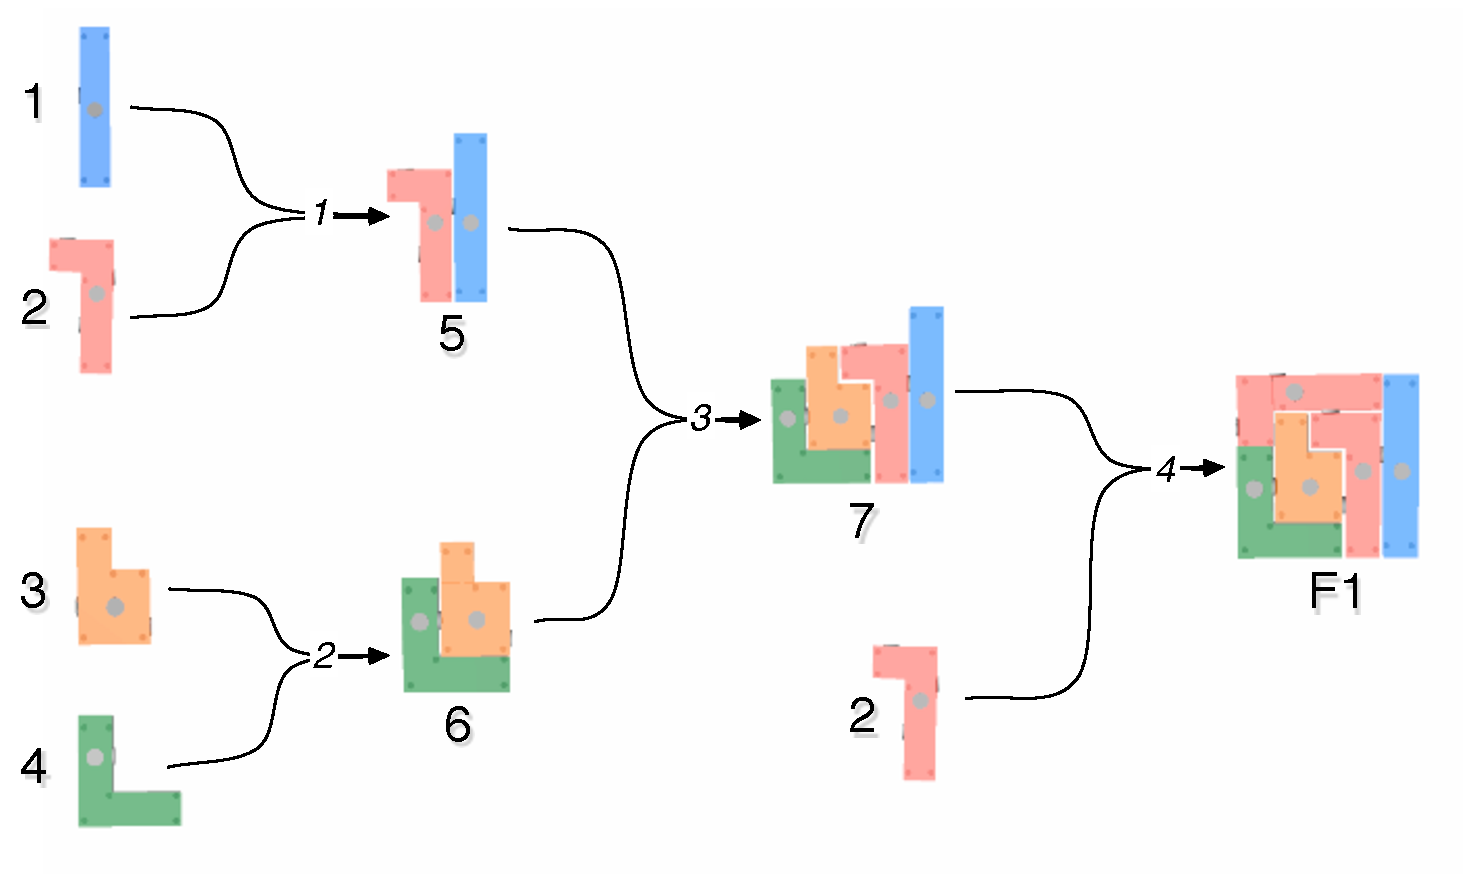
\includegraphics[width=11cm]{img/assembly_plan_f1.pdf}
					\label{fig:assembly_plans:f1}
			 	}
				\; % espacement entre figures. \quad \;
				\subfigure[Second final puzzle plan] 
				{
					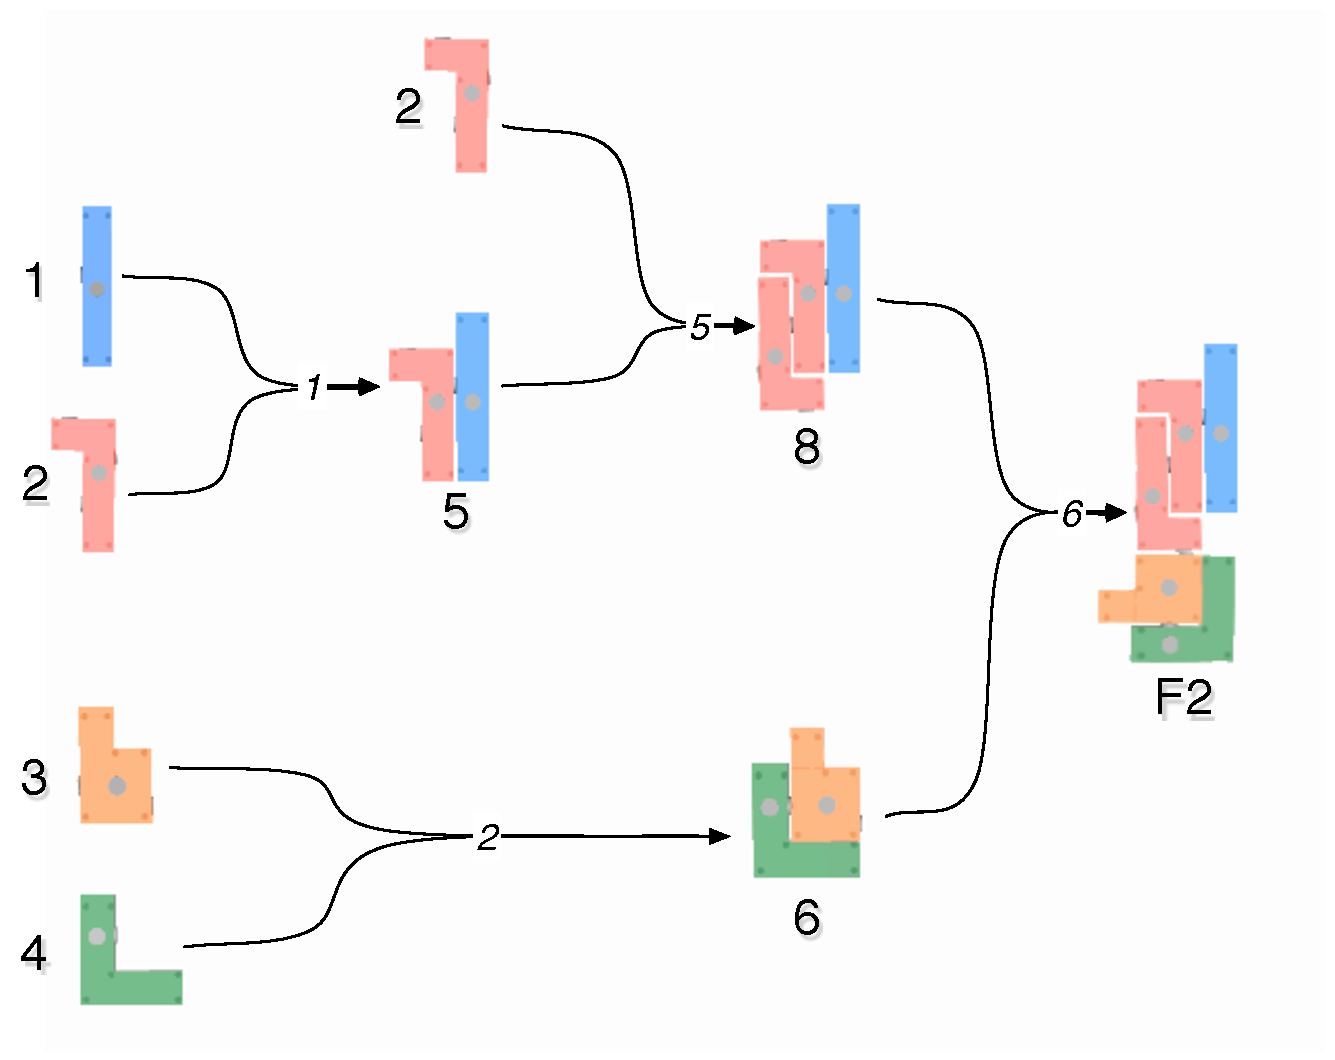
\includegraphics[width=11cm]{img/assembly_plan_f2.pdf}
					\label{fig:assembly_plans:f2}
			 	}
				\caption{Assembly plans for the two final puzzles considered. All groups of connected pieces (mid-assemblies or products) are given an unique name in a form of a number. Arrows show the assembly steps, with their name as number.}
			\label{fig:assembly_plans} %Cation general
			\end{figure}

		% subsubsection assembly_plans (end)
			
	% subsection pieces (end)
	
	\subsection{Robots} % (fold)
	\label{sub:robots}
	For the robots, we used the KheperaIII model available in Webots. It offered a small scale yet not too crude mobile robot for our first implementation.
	
	In order to manipulate the pieces, we equipped the robots with a protruding carrying arm (see Figure~\ref{fig:robot_overview}). This arm consists of a simple bar with a mobile Connector at its end. The Connector is allowed to turn around 360$^{\circ}$ using a rotational Servo, in order to orient the carried piece in any possible direction. The length of the arm is sufficient to rotate any mid-assembly without hitting the robot's body.

	\begin{figure}[h!]
		\centering
		\subfigure[KheperaIII robot.] 
		{
			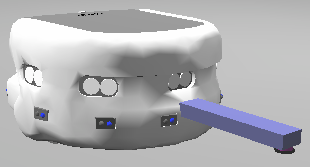
\includegraphics[height=3cm]{img/robot_overview_all.pdf}
			\label{fig:robot_overview_all}
	 	}
		\; % espacement entre figures. \quad \;
		\subfigure[Protruding arm, with rotating connector.] 
		{
			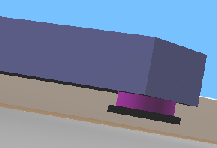
\includegraphics[height=3cm]{img/robot_overview_arm.pdf}
			\label{fig:robot_overview_arm}
	 	}
		\caption{KheperaIII robot model in Webots, with protruding arm.}
	\label{fig:robot_overview} %Cation general
	\end{figure}
	

	When being carried, the piece does not touch the ground, as they are very light-weight.
	
	The robots have similar components to the pieces:
	\begin{my_itemize}
		\item They have a radio emitter/receiver, to communicate with pieces and other robots. The communication range is set to 60cm for the robots. This local radio is also used as a bearing detection mechanism, giving the relative angle between two emitter/receivers. This is used when a robot needs to grab a piece, or when the piece has to be rotated by the rotating arm of a given angle.
		\item They can control the rotation of the servo at the tip of their protruding arm.
		\item They communicate with their carried piece to know what type it is and what is its relative angle.
		\item They know the assembly plans to create the final puzzles.
		\item They move around randomly in the arena, while avoiding other robots and walls using their infra-red distance sensors.
	\end{my_itemize}
	
	\subsubsection{Movement pattern} % (fold)
	\label{ssub:movement_pattern}
	We want our robots to be evenly distributed around the arena in average. This property, the \textit{well-mixed} property, allows us to use non-spatial mathematical models.
	
	\begin{figure}[h!]
		\centering
		\subfigure[Covered space, 3D] 
		{
			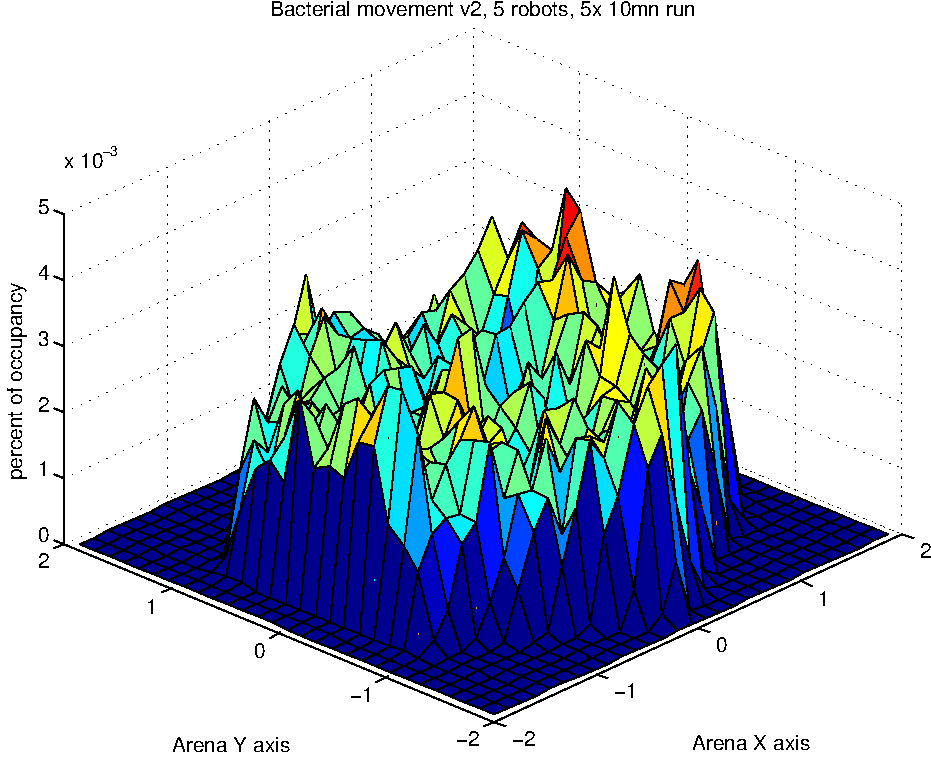
\includegraphics[width=6.5cm]{img/bacterial_covering_3d.pdf}
			\label{fig:img_bacterial_covering_3d}
	 	}
		\; % espacement entre figures. \quad \;
		\subfigure[Covered space, 2D] 
		{
			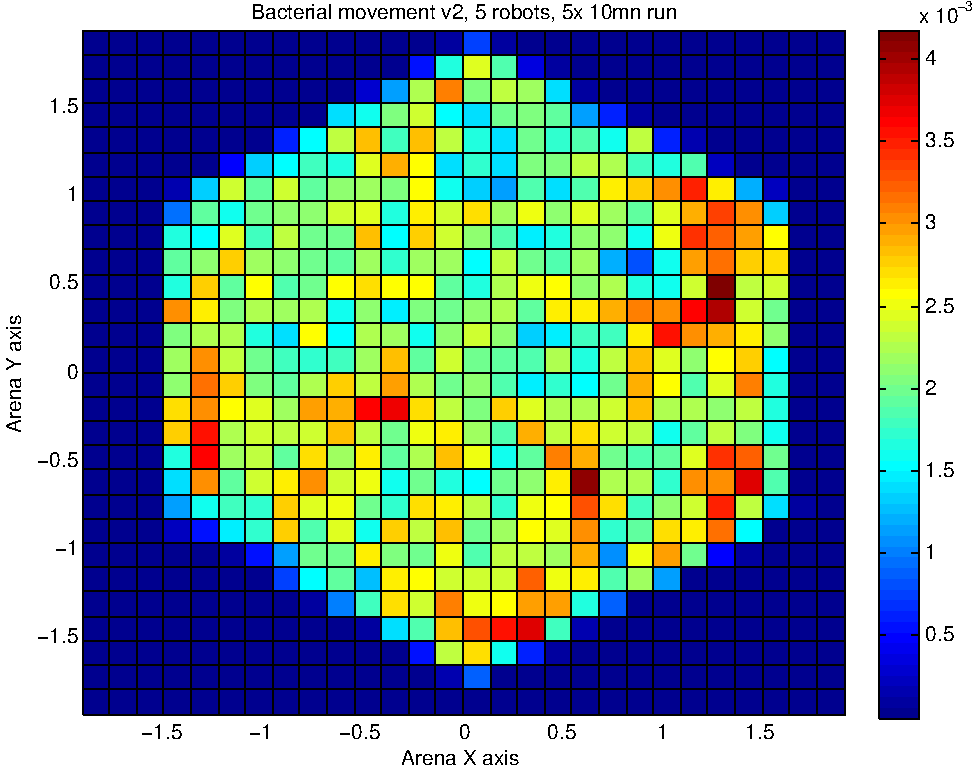
\includegraphics[width=6.5cm]{img/bacterial_covering_2d.pdf}
			\label{fig:img_bacterial_covering_2d}
	 	}
		\caption{Average coverage of the arena by 5 robots moving in a brownian-like motion, over 5 runs of 10 minutes.}
	\label{fig:covering_brownian} %Cation general
	\end{figure}
	
	In order to satisfy this property, the robots have to move around in a specific manner. We chose to make them move in a bacterial-like movement. This movement, ``chemotaxis'', allows bacteria to move around, search for nutriments and avoid dangers. It is based on a forward movement, and random ``tumbling''. A ``tumble'' is a random turn. The bacteria sample the concentration of nutriments or dangerous chemicals, and performs a temporal integration on them while moving. An increase in a nutriments concentration tends to reduce the number of tumbling, promoting movement towards the spacial gradient. When the gradient is constant, the bacteria performs tumbling at a constant rate~\cite{Berg:2000p10058, Adler:1975p7745, Macnab:1972p7813, Dhariwal:1926p7464}.

	In our case, we do not follow any gradient. We only make the robots move forward for a random distance, and then turn randomly around, before moving forward again. This creates a random movement that is supposed to cover more uniformly the space.
	
	We verified this assumption using Webots and our robots. See Figure~\ref{fig:covering_brownian} for the average space covered by five robots over 5 runs of 10 minutes each. We see that the space is nearly evenly covered, which shows that our property is ensured.
	
	
	% subsubsection movement_pattern (end)
	
	\subsubsection{Behavior} % (fold)
	\label{ssub:behavior}
		The robots and the pieces are placed randomly in an hexagonal arena of fixed size. They can only communicate in a local range: 40cm for robot to piece, 60cm for robot to robot. The behavior is then as follows:
		
		\begin{figure}[h]
			\centering
			\; % espacement entre figures. \quad \;
			\subfigure[Encountering between a robot and a piece. The robot aligns itself with the piece.] 
			{
				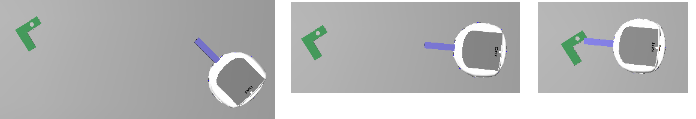
\includegraphics[width=10cm]{img/align_approach_piece.png}
				\label{fig:img_align_approach_piece}
		 	}
			\; % espacement entre figures. \quad \;
			\subfigure[Alignment of piece by the rotating connector] 
			{
				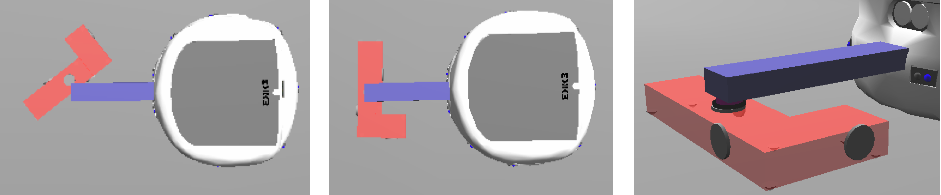
\includegraphics[width=10cm]{img/rotate_piece.png}
				\label{fig:img_rotate_piece}
		 	}
			\; % espacement entre figures. \quad \;
			\subfigure[Approach between two robots and assembling of pieces.] 
			{
				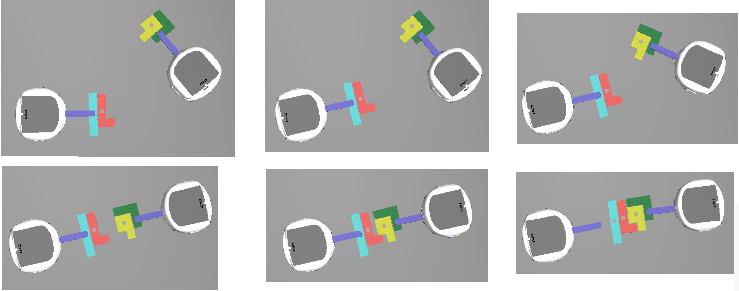
\includegraphics[width=10cm]{img/align_approach.png}
				\label{fig:img_align_approach}
		 	}
			\caption{Assembly behavior of robots and pieces.}
		\label{fig:behavior_webots_assembly} %Cation general
		\end{figure}
		
		
		\begin{my_itemize}
			\item Robots move around, searching for lying pieces. They avoid the walls and other robots using a Braitenberg vehicle controller. The move around randomly following the bacterial-like movement pattern presented before.
			\item Robots and pieces broadcast messages locally, telling their current configuration and state. A configuration is a unique name for a set of assembled pieces, for all possible assemblies present in the plans we are using to build the final puzzles.
			\item When a robot receives a message from a free piece (i.e. they are in a small communication range), it aligns with it, go towards it and carries it. This alignment uses relative range and bearing offered by the emitter/receiver nodes of Webots. See Figure~\ref{fig:img_align_approach_piece}.
			\item While carrying the piece, the robot start moving around again, searching for another robot with a compatible piece. Robots communicate with small range messages broadcasted at all time.
			\item When two robots carrying pieces come into communication ranges, they exchange message and look into the assembly plan. If their pieces correspond to no stored assembly step, they moves away from each other. 
			\item If their pieces can be assembled, the robot start an assembly procedure. According to the piece type and the assembly plan, the robot first orient their pieces so as to show the good connector in front. Again we use the relative range and bearing of emitter/receiver nodes to perform that alignment. This step will be relaxed in a experimental scenario to account for a random orientation of pieces for the assembly. See Figure~\ref{fig:img_rotate_piece}.
			\item Then the robot align each other. The robot starts to approach, allowing the pieces to lock to each other. When the two pieces are locked, one of the robot leaves, letting the other one with the assembled pieces. This robot resume searching for a new piece to assemble with, while the newly freed robot starts looking for a lying piece. See Figure~\ref{fig:img_align_approach}
		\end{my_itemize}
		
	% subsubsection behavior (end)
	
	% subsection robots (end)
	
	\subsection{Experiment platform} % (fold)
	\label{sub:experiment_platform}
	
		Our goal is to reproduce experiments extensively and study the data in Matlab. We thus need a pretty robust system, as well as a centralized way to prepare and store these experiments.
		
		The robustness is ensured by adding several checks and reset capabilities in the behaviors of the robots and pieces. There are still problems that could arise, for example due to physical simulation problems, or a discrepancy between the actual state of the simulation and the way the robots see it. We can only measure what the robots know, so this can create some problems.
		
		As a centralized medium for the experiments, we use a supervisor node in Webots. This supervisor takes care of the experiments and writes the results to different files. It resets the experiments after a maximum elapsed time and takes care of the initial random positions of all pieces and robots. When an assembly step occurs, robots send specific messages to that supervisor, which will save them accordingly.
		
	% subsection experiment_platform (end)
	
	\subsection{Python world generator} % (fold)
	\label{sub:python_world_generator}
		
		Webots does not provide an easy way of varying the components of a given world. However, as we want to control easily the number of robots, pieces, the size of the arena and several other parameters. Therefore, we created our own Webots world generator, in Python.
		
		This world generator is available online on the mailing group of Webots, as it was build to be easily extended. It takes the following inputs:
		
		\begin{my_itemize}
			\item A set of template files. They store parts of a classical Webots VRML world file, but with added free parameters in them.
			\item A input XML file describing the world to create. This file defines which templates to use and how many instances of them to create and finally assigns values to the free parameters.
		\end{my_itemize}
		
		It is easy to add new templates and extend this to different applications.
		
		This generator allows us to generate experimental worlds containing different numbers of pieces and robots easily. We study for now a world with 5 pieces and 4 or 5 robots, and a world with 15 pieces and 15 robots.
		
	% subsection python_world_generator (end)
% section webots_implementation (end)

\section{The robot transporters scenario} % (fold)
\label{sec:the_robot_transporters_scenario}

\paragraph{Characteristics:} % (fold)
\label{par:characteristics_}
Lying pieces, robots carry and assemble them.
% paragraph characteristics_ (end)

This system represents either a self-assembly task if we abstract the robots, or a transporting and assembly task. The pieces can not move and rely on the robots to create a puzzle.

\subsection{Simulation results} % (fold)
\subsubsection{Experiment 1: 5 pieces and 4 robots, final puzzle F1 only} % (fold)
\label{ssub:experiment_1_5_pieces_and_4_robots}

Setup:
\begin{my_itemize}
	\item Hexagonal arena, radius 2m.
	\item 100 experiments.
	\item 20 minutes maximum per experiment.
	\item Pieces and robots initialized at random positions.
	\item Pieces are aligned by the robots before an assembly.
	\item Robots follow the plan to create the final puzzle F1 only, given in Figure~\ref{fig:assembly_plans:f1}.
\end{my_itemize}


\begin{figure}[h!]
	\centering
	% \hspace{-30pt}
	\subfigure[Averaged populations of products over time.] 
	{
		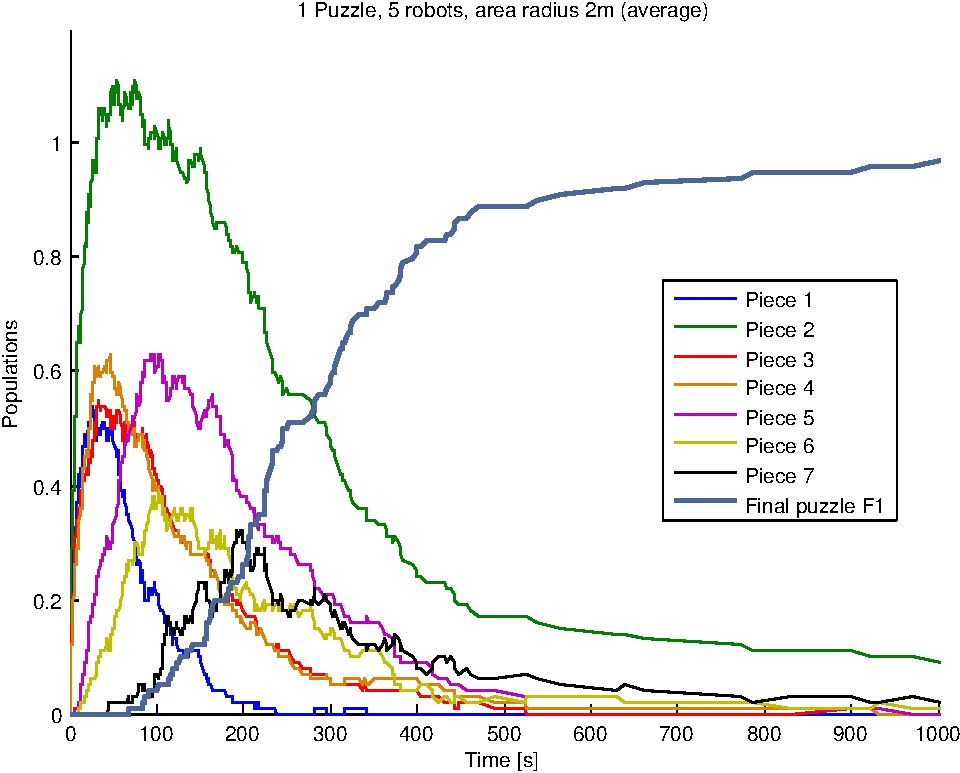
\includegraphics[width=9cm]{img/webots_measure_1puzzle_alone.pdf}
		\label{fig:transporters_experiment1:timeseries}
 	}
	% \; % espacement entre figures. \quad \;
	\subfigure[Histogram of the finishing times of the final puzzles F1. Red line at 400 seconds shows the 75\% quantile.] 
	{
		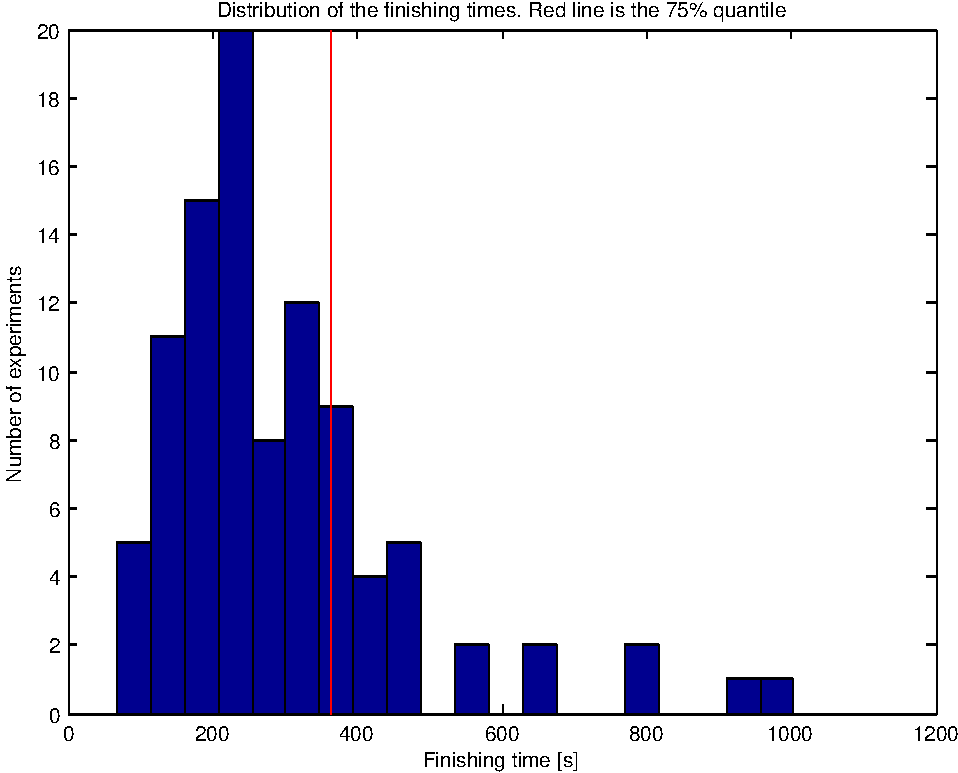
\includegraphics[width=9cm]{img/webots_measure_1puzzle_finishingtimes.pdf}
		\label{fig:transporters_experiment1:finishingtimes}
 	}
	\caption{Physical simulation results for the robot transporter scenario, Experiment 1: 5 pieces, 4 robots and final puzzle F1 only.}
\label{fig:transporters_experiment1} %Cation general
\end{figure}

We see on Figure~\ref{fig:transporters_experiment1:timeseries} that the final puzzle F1 follows an exponential saturating curve, tending toward 1. This is what we expected, as only one puzzle can be created. The curve does not attain exactly 1, meaning that some assemblies are not successful. Indeed, we have a success rate of assembly after 20 minutes of 96\%.

But looking at Figure~\ref{fig:transporters_experiment1:finishingtimes}, which shows the histogram of the times of creation of the final puzzles over all experiments, we see that 75\% of the puzzles are actually completed after 6 minutes and 40 seconds on average. This is a good results, as it means that most of the experiments were completed quickly.

% subsubsection experiment_1_5_pieces_and_4_robots (end)

\subsubsection{Experiment 2: 15 pieces and 15 robots, final puzzle F1 only} % (fold)
\label{ssub:experiment_2_15_pieces_and_15_robots_final_puzzle_f1_only}

Setup:
\begin{my_itemize}
	\item Hexagonal arena, radius 3m.
	\item 100 experiments.
	\item 20 minutes maximum per experiment.
	\item Pieces and robots initialized at random positions.
	\item Pieces are aligned by the robots before an assembly.
	\item Robots follow the plan to create the final puzzle F1 only, given in Figure~\ref{fig:assembly_plans:f1}.
\end{my_itemize}

\begin{figure}[h!]
	\centering
	\subfigure[Averaged populations of products over time.] 
	{
		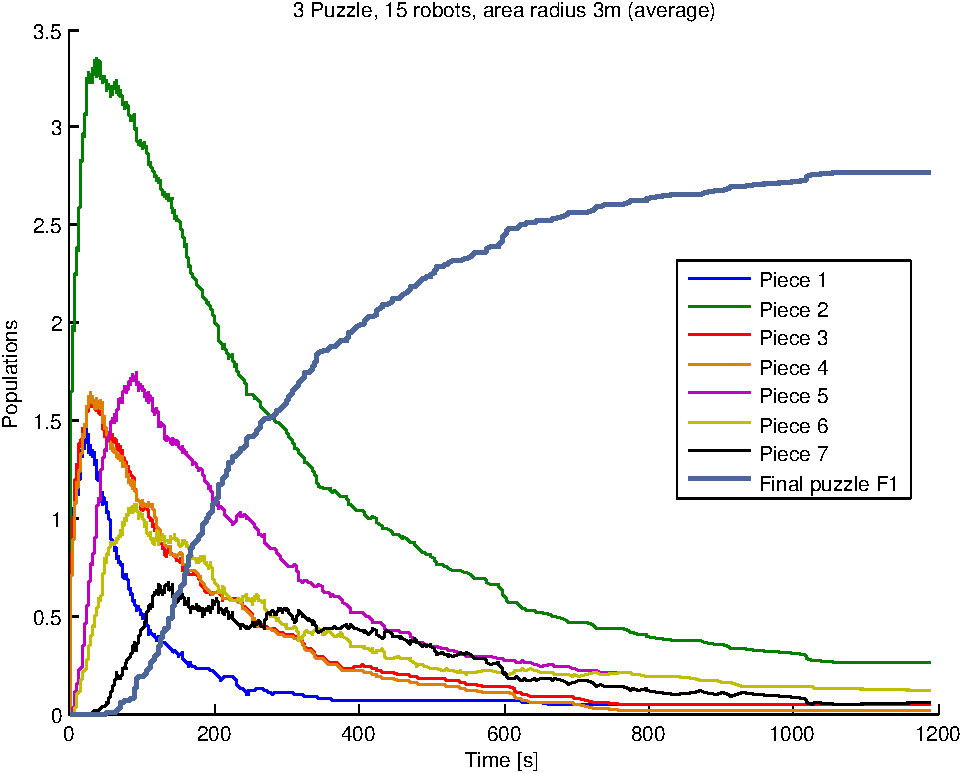
\includegraphics[width=9cm]{img/webots_measure_3puzzle_alone.pdf}
		\label{fig:transporters_experiment2:timeseries}
 	}
	\; % espacement entre figures. \quad \;
	\subfigure[Histogram of the finishing times of the final puzzles F1. Red line at 400 seconds shows the 75\% quantile.] 
	{
		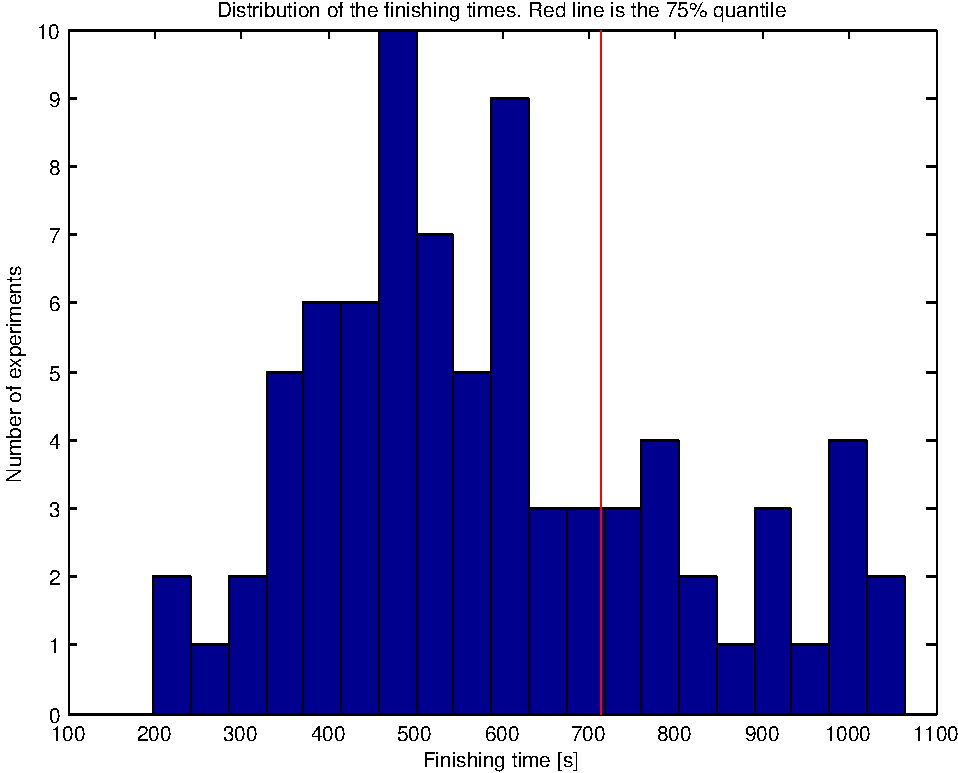
\includegraphics[width=9cm]{img/webots_measure_3puzzle_finishingtimes.pdf}
		\label{fig:transporters_experiment2:finishingtimes}
 	}
	\caption{Physical simulation results for the robot transporter scenario, Experiment 2: 15 pieces, 15 robots and final puzzle F1 only.}
\label{fig:transporters_experiment2} %Cation general
\end{figure}

Figure~\ref{fig:transporters_experiment2:timeseries} shows a similar behavior than before. The curve is smoother, due to the bigger amount of pieces and possible final puzzles. The curve again tends exponentially towards the maximal puzzle number, 3. But it converges to an even smaller number, as more assemblies goes wrong. After 20 minutes, we have a success rate of assembly of 3 puzzles of 80\% only. This shows that some things can still go wrong in our physical simulations, which affects the final assembly yield.

Looking at Figure~\ref{fig:transporters_experiment2:finishingtimes}, we see that the 75\% quantile for the successfully assembled 3 final puzzles is at 11 minutes. This is still a pretty good result, which shows that our approach is scalable to a higher number of pieces and robots, assuming that the space available for the movements does not become too small.

% subsubsection experiment_2_15_pieces_and_15_robots_final_puzzle_f1_only (end)

\subsubsection{Experiment 3: 5 pieces and 5 robots, final puzzles F1 and F2} % (fold)
\label{ssub:experiment_3_5_pieces_and_5_robots_final_puzzles_f1_and_f2}

Setup:
\begin{my_itemize}
	\item Hexagonal arena, radius 2m.
	\item 100 experiments.
	\item 20 minutes maximum per experiment.
	\item Pieces and robots initialized at random positions.
	\item Pieces are aligned by the robots before an assembly.
	\item Robots follow the plans to create the final puzzles F1 and F2. See Figure~\ref{fig:assembly_plans}.
\end{my_itemize}


\begin{figure}[h!]
	\centering
	\subfigure[Averaged populations of products over time.] 
	{
		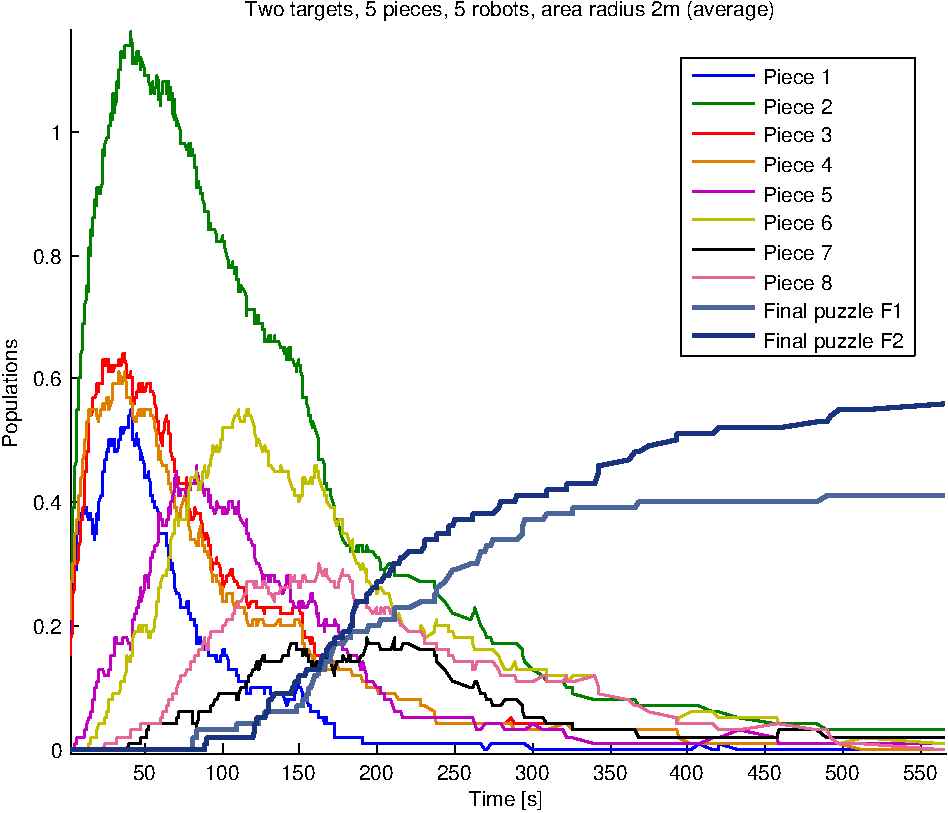
\includegraphics[width=9cm]{img/webots_measure_twotargets_1puzzle_alone.pdf}
		\label{fig:transporters_experiment3:timeseries}
 	}
	\; % espacement entre figures. \quad \;
	\subfigure[Histogram of the finishing times of either final puzzle F1 or F2. Red line at 400 seconds shows the 75\% quantile.] 
	{
		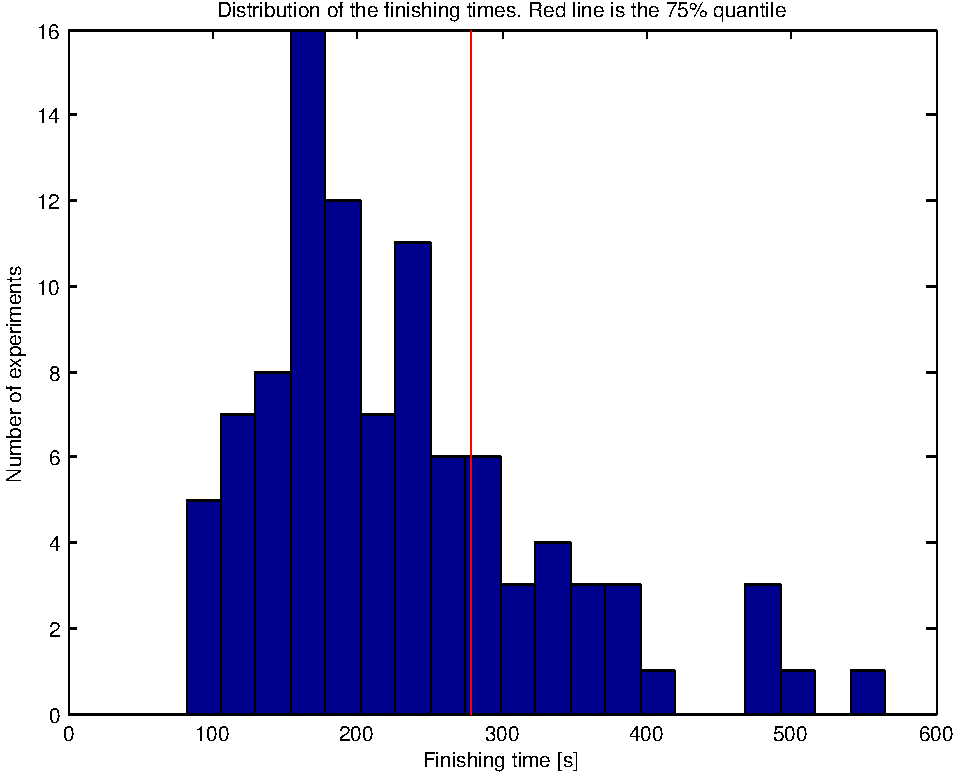
\includegraphics[width=9cm]{img/webots_measure_twotargets_1puzzle_finishingtimes.pdf}
		\label{fig:transporters_experiment3:finishingtimes}
 	}
	\caption{Physical simulation results for the robot transporter scenario, Experiment 3: 5 pieces, 5 robots and final puzzles F1 and F2.}
\label{fig:transporters_experiment3} %Cation general
\end{figure}

Figure~\ref{fig:transporters_experiment3:timeseries} shows an interesting result. We see that the two final puzzle converge to a value that sum (more or less) to $1$. But the distribution between the two assemblies is not even, we have $60\%$ of final puzzle $F2$ and $40\%$ of final puzzle $F1$. By looking at the assembly plans and the available initial pieces, we think it is due to reaction 5. This reaction uses piece 5, which is created early, and uses another piece 2, which is easily available (purple curve and green curve). Compared to reaction 3, which uses a piece 5 and a piece 6, which takes more time to be produced, there is less time dependence on the path to F2. This tends to promote it.

This discrepancy triggered the idea of being able to control the ratio between the two final puzzles, by modifying the system. This will be the subject of our Augmentation step and optimization of the model, Chapter~\ref{cha:chemical_reaction_networks_control_and_design} and \ref{cha:augmented_assembly_implementation}.

From Figure~\ref{fig:transporters_experiment3:finishingtimes}, we see that the 75\% quantile for the successfully assembled final puzzle is at 4 minutes 30 seconds, with a success ratio of $97\%$. This is again very good, few assemblies go bad, even with the two possible final puzzles.
% This is better than for experiment 1, which can be explained by the added robot. 

% subsubsection experiment_3_5_pieces_and_5_robots_final_puzzles_f1_and_f2 (end)

% \subsubsection{Experiment 4: random alignment of pieces before assemblies} % (fold)
% \label{ssub:experiment_4_random_alignment_of_pieces_before_assemblies}
% 
% Setup:
% \begin{my_itemize}
% 	\item Hexagonal arena, radius 2m.
% 	\item 100 experiments.
% 	\item 20 minutes maximum per experiment.
% 	\item Pieces and robots initialized at random positions.
% 	\item Carried pieces are rotated randomly when moving around.
% 	\item The pieces are not aligned before an assembly.
% 	\item Robots follow the plans to create the final puzzles F1 and F2. See Figure~\ref{fig:assembly_plans}.
% \end{my_itemize}
% 
% % subsubsection experiment_4_random_alignment_of_pieces_before_assemblies (end)

% subsection simulation_results (end)
% section the_robot_transporters_scenario (end)

\section{The self-assembling pieces scenario} % (fold)
\label{sec:the_self_assembling_pieces_scenario}
When the pieces can move around and assemble on their own, robots are not necessary anymore. This scenario is closer to a real nano self-assembly task, but at a macro-scale level.

We developed such a scenario in Webots, using the same pieces with several modifications:
\begin{my_itemize}
	\item The pieces are pushed by individual forces, of randomly chosen direction. The pieces have a low friction coefficient with the floor to allow easy movement.
	\item There are forces applied onto the pieces when they approach the walls too closely. This introduce a wall-avoidance in a smooth fashion. The repulsive force $F_r$ applied is directed toward the center of the arena and an amplitude inversely proportional to the current distance to the walls:
	\[
		F_r \sim \frac{1}{\left(\sqrt{x^2+y^2} - R_a sin(\frac{\pi}{3}) \right)^2} \cdot \left( 
		\begin{array}{c} -x \\
			-y \end{array} \right)
	\]
	$R_a sin(\frac{\pi}{3})$ is the radius of the incircle to the hexagonal arena of radius $R_a$. 
	\item The pieces attracts each others in a small radius. This was introduced to improve the encountering rate, which was not comparable to the one we had before. Indeed, a collision of two pieces is less likely than the encountering of two communication circles as we had before. This force attracts the pieces for some time, and then repulse then, to mimic a missed assembly.
\end{my_itemize}

All these modifications create a scenario where the assembly rates are much smaller than before, but which can still create some final puzzles. Unfortunately, due to robustness issues, we did not manage to get systematic experiments in time for that scenario. Its study will be done in further works.

% section the_self_assembling_pieces_scenario (end)

\section{The mixed assembly scenario} % (fold)
\label{sec:the_mixed_assembly_scenario}

We can combine the two last scenarios into this fully complex one. The pieces can move around and assemble on their own, but can also be carried around and assembled by robots.

In order to make the carrying possible, the pieces stop moving when a robot is trying to grab them. Moreover, a free piece cannot interact with a carried piece. The robot has to drop it first.

This scenario closely resembles a biological process with enzymatic components. The pieces assemble following their own dynamics, which are improved by the robots via their specific actions and orientation capabilities.

Again we did not manage to completely study this scenario. We leave it as further work, not without regrets.